%-----------------------------------------------------------------------------%
\chapter{\babEmpat}
%-----------------------------------------------------------------------------%
Pada bab ini, hasil dari pengujian tuning Hypervisor KVM akan dijelaskan. Proses pengujian tersebut melibatkan penggunaan program benchmark yang telah dijelaskan secara rinci pada bab 3. Dalam pengujian ini, \saya\ mengeksplorasi berbagai parameter dan konfigurasi yang dapat diterapkan pada Hypervisor KVM untuk meningkatkan kinerja dan efisiensi sistem secara keseluruhan. Selain itu, \saya\ juga melakukan analisis terhadap data pengujian.

%-----------------------------------------------------------------------------%
\section{Hasil Tuning Hypervisor KVM dengan Kompresi Video}
%-----------------------------------------------------------------------------%
Pada bagian ini akan dijelaskan hasil pengujian tuning Hypervisor KVM dengan menggunakan program benchmark yang telah dibuat sebelumnya dengan melakukan kompresi video.

Dibawah ini merupakan daftar konfigurasi yang digunakan dalam pengujian tuning Hypervisor KVM dengan kompresi video:

\begin{multicols}{2}
    \begin{enumerate}
        \item Default
        \item SSSE3
        \item SSE4.1
        \item SSE4.2
        \item SSE4a
        \item SSSE3+SSE4.1
        \item SSSE3+SSE4.2
        \item SSSE3+SSE4a
        \item SSE4.1+SSE4.2
        \item SSE4.1+SSE4a
        \item SSE4.2+SSE4a
        \item SSSE3+SSE4.1+SSE4.2
        \item SSSE3+SSE4.1+SSE4a
        \item SSSE3+SSE4.2+SSE4a
        \item SSE4.1+SSE4.2+SSE4a
        \item SSSE3+SSE4.1+SSE4.2+SSE4a
    \end{enumerate}
\end{multicols}
\begin{figure}
    \centering
    \caption{Legend Konfigurasi Pengujian Kompresi Video untuk Gambar \ref{fig:video_compression_test_average_graph}}
    \label{fig:video_compression_test_configuration}
\end{figure}

\begin{figure}
    \centering
    \begin{tikzpicture}
        \begin{axis}[
                xbar,
                bar width=2ex,
                xlabel={Detik},
                ytick=data,
                y=3ex,
                nodes near coords,
                nodes near coords align={horizontal},
                symbolic y coords={1,2,3,4,5,6,7,8,9,10,11,12,13,14,15,16},
                enlarge y limits=0.1,
                enlarge x limits=0.1,
                width=\textwidth,
                height=0.6\textheight,
                xmin=0,
                xmax=160,
                grid=major,
                grid style={dashed, black!30},
                axis background/.style={fill=gray!10},
                y axis line style={opacity=0},
                tick,
                yticklabel style={font=\footnotesize},
                xticklabel style={font=\footnotesize},
                xlabel style={font=\normalsize, color=black, font=\bfseries},
            ]
            \addplot[red!20!black,fill=blue!60!white] coordinates {
                    (138.236,1)
                    (123.965,2)
                    (70.7347,3)
                    (137.712,4)
                    (137.801,5)
                    (57.9751,6)
                    (93.2180,7)
                    (123.818,8)
                    (71.0522,9)
                    (70.9115,10)
                    (137.731,11)
                    (58.2748,12)
                    (57.9563,13)
                    (123.737,14)
                    (137.732,15)
                    (57.7008,16)
                };
        \end{axis}
    \end{tikzpicture}
    \caption{Grafik Waktu Rata-rata Pengujian dengan Kompresi Video}
    \label{fig:video_compression_test_average_graph}
\end{figure}

Grafik \ref{fig:video_compression_test_average_graph} menampilkan rata-rata waktu yang dibutuhkan untuk melakukan kompresi video pada berbagai konfigurasi berdasarkan gambar \ref{fig:video_compression_test_configuration}. Dari grafik tersebut, terlihat bahwa konfigurasi dengan waktu rata-rata terlama adalah konfigurasi Default dengan waktu rata-rata 138.24 detik, sedangkan konfigurasi dengan waktu rata-rata tercepat adalah konfigurasi SSSE3 + SSE4.1 + SSE4.2 + SSE4a dengan waktu rata-rata 57.7 detik.

\begin{figure}
    \centering
    \begin{tikzpicture}
        \begin{axis}[
                xbar,
                bar width=2ex,
                xlabel={\f{Speedup}},
                ytick=data,
                y=3ex,
                nodes near coords,
                nodes near coords align={horizontal},
                symbolic y coords={1,2,3,4,5,6,7,8,9,10,11,12,13,14,15,16},
                enlarge y limits=0.1,
                enlarge x limits=0.1,
                width=\textwidth,
                height=0.6\textheight,
                xmin=0,
                xmax=2.5,
                grid=major,
                grid style={dashed, black!30},
                axis background/.style={fill=gray!10},
                y axis line style={opacity=0},
                tick,
                yticklabel style={font=\footnotesize},
                xticklabel style={font=\footnotesize},
                xlabel style={font=\normalsize, color=black, font=\bfseries},
            ]
            \addplot[red!20!black,fill=blue!60!white] coordinates {
                    (1.0000,1)
                    (1.115,2)
                    (1.954,3)
                    (1.003,4)
                    (1.003,5)
                    (2.384,6)
                    (1.482,7)
                    (1.116,8)
                    (1.945,9)
                    (1.950,10)
                    (1.003,11)
                    (2.372,12)
                    (2.385,13)
                    (1.117,14)
                    (1.003,15)
                    (2.395,16)
                };
        \end{axis}
    \end{tikzpicture}
    \caption{Grafik \f{speedup} Tes Kompresi Video}
    \label{fig:video_compression_test_graph}
\end{figure}

Grafik \ref{fig:video_compression_test_graph} menampilkan \f{speedup} dari berbagai konfigurasi berdasarkan gambar gambar \ref{fig:video_compression_test_configuration}. Dari grafik tersebut, terlihat bahwa konfigurasi dengan \f{speedup} tertinggi adalah SSSE3 + SSE4.1 + SSE4.2 + SSE4a dengan nilai \f{speedup} 2.4, disertai dengan rata-rata waktu kompresi selama 57.7 detik. Keempat flag ini memberikan peningkatan performa yang signifikan untuk melakukan kompresi video. Namun jika dilihat dari hasil lainnya, flag yang sangat berpengaruh adalah SSSE3 dan SSE4.1, dimana untuk SSSE3 saja memiliki nilai \f{speedup} sebesar 1.12, dan untuk SSE4.1 saja memiliki nilai \f{speedup} paling besar yaitu di 1.95. SSSE3 memberikan peningkatan performa karena fiturnya yang dirancang khusus untuk HD audio/video decoding/encoding, sementara SSE4.1 menambahkan instruksi baru seperti \texttt{MPSADBW}, penting untuk beberapa codec \f{High Definition}, dan memungkinkan perhitungan perbedaan blok 8×8 dalam waktu kurang dari tujuh siklus.

%-----------------------------------------------------------------------------%
\section{Hasil Tuning Hypervisor KVM dengan Validasi Integritas Data}
%-----------------------------------------------------------------------------%
Pada bagian ini akan dijelaskan hasil pengujian tuning hypervisor KVM dengan validasi integritas data dengan menggunakan program benchmark kode \ref{code:kode_pengujian_validasi_integritas_data}.

Flag yang digunakan untuk konfigurasi dalam pengujian tuning Hypervisor KVM dengan validasi integritas data adalah SSE4.2.

\begin{figure}
    \centering
    \begin{tikzpicture}
        \begin{axis}[
                xbar,
                bar width=2ex,
                xlabel={Milisecond},
                ytick=data,
                y=3ex,
                nodes near coords,
                nodes near coords align={horizontal},
                symbolic y coords={Default,SSE4.2},
                enlarge y limits=1,
                enlarge x limits=0.1,
                width=\textwidth,
                height=0.6\textheight,
                xmin=0,
                xmax=4.5,
                grid=major,
                grid style={dashed, black!30},
                axis background/.style={fill=gray!10},
                y axis line style={opacity=0},
                tick,
                yticklabel style={font=\footnotesize},
                xticklabel style={font=\footnotesize},
                xlabel style={font=\normalsize, color=black, font=\bfseries},
            ]
            \addplot[red!20!black,fill=blue!60!white] coordinates {
                    (4.1642,Default)
                    (0.5451,SSE4.2)
                };
        \end{axis}
    \end{tikzpicture}
    \caption{Grafik Waktu Rata-rata Pengujian dengan Validasi Integritas Data}
    \label{fig:file_integrity_test_average_graph}
\end{figure}

Grafik \ref{fig:file_integrity_test_average_graph} menunjukkan rata-rata waktu yang dibutuhkan untuk melakukan validasi integritas data pada berbagai konfigurasi yang diuji. Dari grafik tersebut, terlihat bahwa konfigurasi dengan waktu rata-rata terlama adalah konfigurasi Default dengan waktu rata-rata 4.16 ms, sedangkan konfigurasi dengan waktu rata-rata tercepat adalah konfigurasi SSE4.2 dengan waktu rata-rata 0.55 ms.

\begin{figure}
    \centering
    \begin{tikzpicture}
        \begin{axis}[
                xbar,
                bar width=2ex,
                xlabel={\f{Speedup}},
                ytick=data,
                y=3ex,
                nodes near coords,
                nodes near coords align={horizontal},
                symbolic y coords={Default,SSE4.2},
                enlarge y limits=1,
                enlarge x limits=0.1,
                width=\textwidth,
                height=0.6\textheight,
                xmin=0,
                xmax=8,
                grid=major,
                grid style={dashed, black!30},
                axis background/.style={fill=gray!10},
                y axis line style={opacity=0},
                tick,
                yticklabel style={font=\footnotesize},
                xticklabel style={font=\footnotesize},
                xlabel style={font=\normalsize, color=black, font=\bfseries},
            ]
            \addplot[red!20!black,fill=blue!60!white] coordinates {
                    (1.000,Default)
                    (7.563,SSE4.2)
                };
        \end{axis}
    \end{tikzpicture}
    \caption{Grafik \f{speedup} Tes Validasi Integritas Data}
    \label{fig:file_integrity_test_graph}
\end{figure}

Grafik \ref{fig:file_integrity_test_graph} menunjukkan \f{speedup} dari setiap konfigurasi yang diuji. Dari grafik tersebut, dapat dilihat bahwa konfigurasi yang memiliki \f{speedup} tertinggi adalah konfigurasi SSE4.2 dengan nilai \f{speedup} 7.56, dengan rata-rata waktu untuk melakukan validasi integritas data selama 0.55 ms. Flag SSE4.2 terbukti meningkatkan performa dalam perhitungan CRC32 karena SSE4.2 memiliki fungsi yang dibuat secara khusus untuk melakukan perhitungan CRC32.

%-----------------------------------------------------------------------------%
\section{Hasil Tuning Hypervisor KVM dengan Enkripsi dan Dekripsi AES}
%-----------------------------------------------------------------------------%
Pada bagian ini akan dijelaskan hasil pengujian tuning hypervisor KVM dengan enkripsi AES dengan menggunakan program benchmark kode \ref{code:pengujian_enkripsi_aes}.

Flag yang digunakan untuk konfigurasi dalam pengujian tuning Hypervisor KVM dengan enkripsi dan dekripsi AES adalah AES-NI.

\begin{figure}
    \centering
    \begin{tikzpicture}
        \begin{axis}[
                xbar,
                bar width=2ex,
                xlabel={Microsecond},
                ytick=data,
                y=3ex,
                nodes near coords,
                nodes near coords align={horizontal},
                symbolic y coords={Default,AES},
                enlarge y limits=1,
                enlarge x limits=0.1,
                width=\textwidth,
                height=0.6\textheight,
                xmin=0,
                xmax=22,
                grid=major,
                grid style={dashed, black!30},
                axis background/.style={fill=gray!10},
                y axis line style={opacity=0},
                tick,
                yticklabel style={font=\footnotesize},
                xticklabel style={font=\footnotesize},
                xlabel style={font=\normalsize, color=black, font=\bfseries},
            ]
            \addplot[red!20!black,fill=blue!60!white] coordinates {
                    (17.15,Default)
                    (8.18,AES)
                };
        \end{axis}
    \end{tikzpicture}
    \caption{Grafik Rata-Rata Waktu Tes Enkripsi AES}
    \label{fig:aes_encrypt_test_average_graph}
\end{figure}

\begin{figure}
    \centering
    \begin{tikzpicture}
        \begin{axis}[
                xbar,
                bar width=2ex,
                xlabel={Microsecond},
                ytick=data,
                y=3ex,
                nodes near coords,
                nodes near coords align={horizontal},
                symbolic y coords={Default,AES},
                enlarge y limits=1,
                enlarge x limits=0.1,
                width=\textwidth,
                height=0.6\textheight,
                xmin=0,
                xmax=22,
                grid=major,
                grid style={dashed, black!30},
                axis background/.style={fill=gray!10},
                y axis line style={opacity=0},
                tick,
                yticklabel style={font=\footnotesize},
                xticklabel style={font=\footnotesize},
                xlabel style={font=\normalsize, color=black, font=\bfseries},
            ]
            \addplot[red!20!black,fill=blue!60!white] coordinates {
                    (21.4,Default)
                    (8,AES)
                };
        \end{axis}
    \end{tikzpicture}
    \caption{Grafik Rata-Rata Waktu Tes Dekripsi AES}
    \label{fig:aes_decrypt_test_average_graph}
\end{figure}

Grafik \ref{fig:aes_encrypt_test_average_graph} dan \ref{fig:aes_decrypt_test_average_graph} menunjukkan rata-rata waktu yang dibutuhkan untuk melakukan enkripsi dan dekripsi AES pada berbagai konfigurasi yang diuji. Dari grafik tersebut, terlihat bahwa konfigurasi dengan waktu rata-rata terlama adalah konfigurasi Default dengan waktu rata-rata 17.15 $\mu$s untuk enkripsi dan 21.4 $\mu$s untuk dekripsi, sedangkan konfigurasi dengan waktu rata-rata tercepat adalah konfigurasi AES dengan waktu rata-rata 8.18 $\mu$s untuk enkripsi dan 8 $\mu$s untuk dekripsi.

\begin{figure}
    \centering
    \begin{tikzpicture}
        \begin{axis}[
                xbar,
                bar width=2ex,
                xlabel={\f{Speedup}},
                ytick=data,
                y=3ex,
                nodes near coords,
                nodes near coords align={horizontal},
                symbolic y coords={Default,AES},
                enlarge y limits=1,
                enlarge x limits=0.1,
                width=\textwidth,
                height=0.6\textheight,
                xmin=0,
                xmax=3,
                grid=major,
                grid style={dashed, black!30},
                axis background/.style={fill=gray!10},
                y axis line style={opacity=0},
                tick,
                yticklabel style={font=\footnotesize},
                xticklabel style={font=\footnotesize},
                xlabel style={font=\normalsize, color=black, font=\bfseries},
            ]
            \addplot[red!20!black,fill=blue!60!white] coordinates {
                    (1.000,Default)
                    (2.096,AES)
                };
        \end{axis}
    \end{tikzpicture}
    \caption{Grafik \f{speedup} Tes Enkripsi AES}
    \label{fig:aes_encrypt_test_graph}
\end{figure}

\begin{figure}
    \centering
    \begin{tikzpicture}
        \begin{axis}[
                xbar,
                bar width=2ex,
                xlabel={\f{Speedup}},
                ytick=data,
                y=3ex,
                nodes near coords,
                nodes near coords align={horizontal},
                symbolic y coords={Default,AES},
                enlarge y limits=1,
                enlarge x limits=0.1,
                width=\textwidth,
                height=0.6\textheight,
                xmin=0,
                xmax=3,
                grid=major,
                grid style={dashed, black!30},
                axis background/.style={fill=gray!10},
                y axis line style={opacity=0},
                tick,
                yticklabel style={font=\footnotesize},
                xticklabel style={font=\footnotesize},
                xlabel style={font=\normalsize, color=black, font=\bfseries},
            ]
            \addplot[red!20!black,fill=blue!60!white] coordinates {
                    (1.000,Default)
                    (2.675,AES)
                };
        \end{axis}
    \end{tikzpicture}
    \caption{Grafik \f{speedup} Tes Dekripsi AES}
    \label{fig:aes_decrypt_test_graph}
\end{figure}

Grafik \ref{fig:aes_encrypt_test_graph} dan \ref{fig:aes_decrypt_test_graph} memperlihatkan \textit{speedup} dari berbagai konfigurasi yang diuji. Dari grafik tersebut, dapat disimpulkan bahwa konfigurasi dengan \textit{speedup} tertinggi adalah dengan konfigurasi penambahan flag AES yang mencapai \textit{speedup} 2.1 untuk proses enkripsi dan 2.68 untuk proses dekripsi, dengan rata-rata waktu masing-masing 8.18 $\mu$s untuk enkripsi dan 8 $\mu$s untuk dekripsi. Penggunaan flag AES terbukti efektif dalam meningkatkan kinerja pada proses enkripsi dan dekripsi karena AES menyediakan fungsi-fungsi seperti \textit{AESENC} dan \textit{AESENCLAST} yang mendukung proses enkripsi, serta fungsi \textit{AESDEC} dan \textit{AESDECLAST} yang mendukung proses dekripsi. Selain itu, terdapat juga fungsi \textit{AESKEYGENASSIST} yang membantu dalam pembuatan kunci, semuanya dirancang secara khusus untuk mendukung proses enkripsi dan dekripsi menggunakan algoritma AES.